% !TEX program = XeLaTeX
% !TEX encoding = UTF-8
\documentclass[UTF8,nofonts]{article}
%{ctexart}

%\setCJKmainfont[BoldFont=FandolSong-Bold.otf,ItalicFont=FandolKai-Regular.otf]{FandolSong-Regular.otf}
%\setCJKsansfont[BoldFont=FandolHei-Bold.otf]{FandolHei-Regular.otf}
%\setCJKmonofont{FandolFang-Regular.otf}
\RequirePackage{etex}

\usepackage{url}
\usepackage{cancel}
\usepackage{xspace}
\usepackage{graphicx}
\usepackage{multicol}
\usepackage{multirow}
\usepackage{subfig}
\usepackage{amsmath}
\usepackage{amssymb}
\usepackage[a4paper, width=186mm, top=18mm, bottom=18mm, includeheadfoot]{geometry}
%\usepackage[a4paper, width=140mm, top=18mm, bottom=22mm, includeheadfoot]{geometry}
\usepackage{booktabs}
\usepackage{array}
\usepackage{verbatim}
\usepackage{caption}
\usepackage{natbib}
\usepackage{booktabs}
\usepackage{float}
\usepackage{pdflscape}
\usepackage{mathtools}
\usepackage[usenames, dvipsnames]{xcolor}
\usepackage{afterpage}
\usepackage{pgf}
\usepackage{tikz}
\usepackage{dirtree}
\usepackage[style=american]{csquotes}
\usepackage{amsfonts}
\usepackage{tikz}
\usepackage{tkz-graph}
\usetikzlibrary{arrows,decorations.pathmorphing,automata,positioning,backgrounds,fit,shapes.symbols,chains,intersections}

\newtheorem{definition}{Definition}[section]
\newtheorem{theorem}{Theorem}[section]
\newtheorem{lemma}{Lemma}
\newtheorem{proof}{Proof} [section]



\usepackage[toc, page, title, titletoc, header]{appendix}
\usepackage{marginnote}
\usepackage{tablefootnote}

%\renewcommand\appendixname{附\ 录}
%\renewcommand\appendixpagename{附\ 录}
%\renewcommand\appendixtocname{附\ 录}
\renewcommand\abstractname{Abstract}


\usepackage{perpage} %the perpage package
\MakePerPage{footnote} %the perpage package command

\usetikzlibrary{shapes.geometric}%
\usepackage{color}
%\usepackage[pages=some, placement=top]{background}
\usepackage{eso-pic}
\usepackage[final]{pdfpages}

%\includepdf[pages=1]{cover}
\hyphenpenalty=750

\title{\textbf{Loopring:}\\\textbf{Un Protocollo di Scambio Token Decentralizzato}}
\author{
  Daniel Wang\\
  \texttt{daniel@loopring.org}\\
  \and
  	Jay Zhou\\
  	\texttt{jay@loopring.org}\\
  	\and
  	Alex Wang\\
  	\texttt{alex@loopring.org}\\
  	\and
  	Matthew Finestone\\
  	\texttt{matt.finestone@gmail.com}\\
  \\
  \texttt{https://loopring.org}
 }

\makeatletter
\def\CTEX@section@format{\Large\bfseries}
\makeatother

\makeatletter
\newenvironment{tablehere}
 {\def\@captype{table}}
 {}

\newenvironment{figurehere}
 {\def\@captype{figure}}
 {}
\makeatother
%
%\newcommand\BackgroundPic{%
%\put(0, 0){%
%\parbox[b][\paperheight]{\paperwidth}{%
%\vfill
%\centering
%\includegraphics[width=\paperwidth, height=\paperheight, %
%%keepaspectratio]{images/background.jpg}%
%]{images/background.jpg}%
%\vfill
%}}}


\begin{document}
%\AddToShipoutPicture{\BackgroundPic}
\maketitle


\begin{abstract}
Loopring \'e un protocollo aperto per l'implementazione di Exchange decentralizzati. Loopring opera mediante un set pubblico di smart contracts responsabili di scambio e liquidazione, contando inoltre su di un insieme di attori off-chain responsabili dell'aggregazione e comunicazione degli ordini. Il protocollo \'e gratuito, espandibile, e funge da elemento standard portante per la costruzione di applicazioni decentralizzate (dApps) che incorporano la funzionalit\'a di Exchange. I suoi standard interoperabili permettono di effettuare trading in modo anonimo e trustless. Un importante miglioramento rispetto agli attuali protocolli di Exchange decentralizzati \'e rappresentato dal fatto che gli ordini qui possono anche essere combinati ed abbinati ad altri ordini dissimili, ovviando al vincolo rappresentato dalla necessit\'a di costituire delle coppie di scambio tra due tokens e aumentando drasticamente la liquidit\'a. Loopring implementa inoltre una robusta soluzione per la prevenzione del front-running: il tentativo scorretto che consiste nell'invio ad un block di una richiesta di processamento di transazioni in modo pi\'u rapido della stessa soluzione originaria. Loopring \'e agnostico riguardo alla Blockchain d'implementazione, permettendo di fatto un'implementazione su qualsiasi Blockchain che supporti la funzionalit\'a di smart contracts. Al momento attuale, risulta operativo su Ethereum \cite{buterin2017ethereum} \cite{wood2014ethereum} e Qtum \cite{dai2017smart}, con NEO \cite{atterlonn2018distributed} in corso d'implementazione.

\end{abstract}



\begin{multicols}{2}
\section{Introduzione\label{sec:introduction}}

 Con la proliferazione dei beni  basati sulla blockchain, il bisogno di scambiare tali beni tra controparti \'e incrementato significativamente. L'introduzione di migliaia di nuovi tokens - che comprende anche la tokenizzazione dei beni tradizionali -  ha fatto s\'i che questo bisogno si amplificasse. Sia che si scambino tokens per motivazioni di trading speculativo, o che vengano convertiti in token d'utilizzo per accedere a networks specifici, la capacit\'a di scambiare un bene crypto per un altro costituisce le fondamenta di un ecosistema pi\'u grande. Difatti, questi beni  possiedono una potenziale energia \cite{desotocapital}, tuttavia liberare questa energia - sbloccare capitali - richiede non solo di determinare la propriet\'a, cosa che la blockchain ha immutabilmente consentito di fare, ma anche l'abilit\'a di trasferire e trasformare liberamente questi beni.

 In questo modo, lo scambio di tokens che non richiedono un rapporto di fiducia, \'e un caso d'uso convincente per la tecnologia blockchain. Tuttavia, fino ad ora, gli appassionati di cripto-beni si sono in larga parte accontentati di scambiare tokens in exchanges centralizzati tradizionali. Il protocollo di Loopring \'e necessario perch\'e, cos\'i come coscienziosamente Bitcoin \cite{nakamoto2008bitcoin} ha enfatizzato, a proposito di denaro elettronico peer-to-peer, \enquote{i maggiori benefici sono persi se una terza parte fidata \'e ancora necessaria per prevenire la doppia spesa}, allo stesso modo, i principali benefici delle risorse decentralizzate sono perduti se devono passare attraverso exchanges fidati, chiusi e centralizzati.

Scambiare tokens decentralizzati su exchanges centralizzati perde di significato dal punto di vista filosofico, considerando che fallisce nel supportare i valori che questi progetti decentralizzati sposano. Vi sono numerosi rischi pratici e limitazioni nell'uso di exchanges che saranno descritti in seguito. Gli exchanges Decentralizzati (DEXs) \cite{schuh2015bitshares} \cite{bancor} \cite{kyber} hanno cercato di affrontare questi problemi, e in molti casi sono riusciti a mitigare i rischi per la sicurezza usando la blockchain per trattative dirette. Tuttavia, mentre le competenze di DEX stanno diventando infrastrutture cruciali per la new economy, vi \'e un significativo spazio di manovra per migliorarne le prestazioni. Loopring ha lo scopo di fornire strumenti modulari per la suddetta infrastruttura con il suo  protocollo dApp aperto e agnostico.

\section{L'Attuale Panorama degli Exchange\label{sec:current_exchange_landscape}}

\subsection{Inadeguatezze degli Exchanges Centralizzati}
I tre rischi primari degli exchange centralizzati sono;	1) Mancanza di sicurezza, 2) Mancanza di trasparenza, 3) Mancanza di liquidit\'a.

\textbf{La mancanza di Sicurezza} sorge generalmente da utenti che consegnano il controllo delle loro chiavi private (quindi dei fondi) ad un'entit\'a centralizzata. Ci\'o, espone gli utenti alla possibilit\'a che gli exchange centralizzati cadano preda di hackers. I rischi sulla sicurezza e di attacco informatico di cui soffrono gli exchanges sono ben noti\cite{coincheckhack}  \cite{mcmillan2014inside}, nonostante ci\'o sono spesso accettati come fattori indispensabili nello scambio di token.  Gli exchanges centralizzati continuano ad essere attraenti per gli hackers, che seguitano negli attacchi ai server i quali custodiscono milioni di dollari di fondi di utenti. Inoltre, gli sviluppatori di exchange possono anche commettere errori accidentali, in buonafede, con i fondi degli utenti. Semplicemente, gli utenti non sono in controllo dei loro tokens quando li depositano in un exchange centralizzato.

\textbf{La mancanza di Trasparenza} espone gli utenti al rischio che exchanges disonesti si comportino in maniera scorretta. La distinzione sta nelle intenzioni malevole degli operatori degli exchanges, dato che gli utenti non scambiano realmente i loro beni negli exchange centralizzati, bens\'i un IOU. Quando i tokens sono spediti al wallet dell'exchange, l'exchange li prende in custodia e offre un IOU al loro posto. Tutti gli scambi sono quindi effettuati con IOUs tra utenti. Per prelevare, gli utenti riscattano i loro IOU dall'exchange e ricevono in cambio i tokens sull'indirizzo del loro wallet esterno. In questo processo vi \'e una carenza di trasparenza e l'exchange pu\'o chiudere, congelare il tuo account, dichiarare bancarotta etc. Sussiste anche la possibilit\'a che utilizzino i beni degli utenti per altri scopi mentre li tengono in custodia, come ad esempio prestarli a terze parti. La mancanza di trasparenza pu\'o costare agli utenti a prescindere dalla totale perdita di fondi, ad esempio si pu\'o concretizzare in pi\'u alte commissioni di scambio, ritardi nei momenti di picco di domanda, rischi legati a regolamentazioni e che gli ordini siano oggetto di front running

\textbf{Mancanza di Liquidit\'a.} Dal punto di vista degli operatori degli exchange, la liquidit\'a frammentata impedisce l'ingresso di nuovi exchanges dovuta alla presenza di due scenari in cui il vincitore prende tutto . Nel primo, l'exchange con il pi\'u alto numero di coppie di scambio vince, perch\'e gli utenti trovano pi\'u vantaggioso effettuare tutti gli scambi su un unico exchange. Nel secondo, l'exchange con il pi\'u grande registro delle commesse vince, ci\'o \'e dovuto allo spread denaro-lettera favorevole per ognuna delle coppie di scambio. Questo, scoraggia la competizione dei nuovi arrivati perch\'e diventa difficile per loro accumulare la liquidit\'a iniziale necessaria. Il risultato \'e che molti exchange controllano una grande porzione di mercato nonostante le lamentele degli utenti e sostanziali incidenti di attacchi informatici da parte di hackers. \'E importante sottolineare che pi\'u gli exchange centralizzati si accaparrano porzioni di mercato, pi\'u sono esposti ad attacchi di hackers.

Dal punto di vista degli utenti, la liquidit\'a frammentata riduce sostanzialmente l'esperienza del fruitore. In un exchange centralizzato, gli utenti possono solo scambiare all'interno della disponibilit\'a dell'exchange stesso contro il suo stesso registro delle commesse e tra le coppie di tokens supportati. Per scambiare il token \verb|A| per il token \verb|B|, gli utenti devono andare in un exchange che supporta entrambi i token o registrarsi in exchange diversi, divulgando informazioni personali. Gli utenti spesso hanno bisogno di eseguire scambi preliminari o intermedi, generalmente tra BTC o ETH, pagando uno spread denaro-lettera nel processo. Infine, il registro delle commesse potrebbe non avere sufficiente disponibilit\'a per completare lo scambio senza un materiale rallentamento. Anche se l'exchange afferma di processare grandi volumi non c'\'e garanzia che questo volume e questa liquidit\'a non siano dei falsi \cite{fakevolume}.

Il risultato \'e un disconnesso silos di liquidit\'a e un ecosistema frammentato che assomiglia al vecchio sistema finanziario, con un significativo volume di scambio centralizzato su pochi exchange. La liquidit\'a globale promessa dalla blockchain non ha nessun valore all'interno degli exchange centralizzati.

\subsection{Inadeguatezze degli Exchange Decentralizzati}
Gli exchange decentralizzati differiscono dagli exchange centralizzati in parte perch\'e gli utenti mantengono il controllo delle loro chiavi private (dei loro beni) attraverso l'esecuzione diretta degli scambi sulla blockchain sottostante. Facendo leva sulla stessa tecnologia trustless delle criptovalute, sono riusciti a  mitigare con successo molti dei sopracitati problemi di sicurezza. Tuttavia, i problemi persistono riguardo alla prestazione e alle limitazioni strutturali.

La liquidit\'a spesso resta un problema, dato che gli utenti devono ricercare controparti all'interno di riserve di liquidit\'a e standard eterogenei. Gli effetti della liquidit\'a frammentata si palesano se DEXs o dApps non utilizzano standard consistenti di interoperabilit\'a, o se gli ordini non sono condivisi/propagati all'interno di un ampio network. La liquidit\'a di un registro di commesse (order books) su scambi a prezzo limitato, e specificatamente la sua capacit\'a di  recupero - quanto velocemente gli ordini eseguiti vengono sostituiti da nuovi ordini - pu\'o avere un impatto considerevole sulle strategie di scambio ottimali \cite{limitorderliquidity}. L'assenza di questi standard ha avuto il risultato non solo di ridurre la liquidit\'a, ma anche di esporre gli utenti a smart contracts proprietari con potenziali falle di sicurezza.

Inoltre, visto che gli scambi sono effettuati on-chain, i DEXs ereditano le limitazioni della blockchain su cui sono costruiti, nominalmente: scalabilit\'a, ritardi in esecuzione (mining), e costose modifiche agli ordini. Quindi il registro delle commesse della blockchain non scala particolarmente bene, in quanto eseguire codice sulla blockchain causa un costo (gas), rendendo cancellazioni multiple di ordini proibitivamente costoso. .

Infine, dato che i registri delle commesse della blockchain sono pubbliche, la transazione per collocare un ordine \'e visibile ai minatori nel frattempo che aspetta di essere minato nel prossimo blocco e piazzato in un registro di commissioni. Questo ritardo espone gli utenti al rischio di front running e di ritrovarsi il prezzo o l'esecuzione rivolto contro di lui.

\subsection{Soluzioni Ibride}
Per le ragioni sopracitate, gli exchange basati puramente sulla blockchain presentano delle limitazioni che li rende non competitivi rispetto agli exchange centralizzati.  Esiste un trade-off tra la propriet\'a di assenza di fiducia caratteristica delle soluzioni on-chain  e la velocit\'a e flessibilit\'a degli ordini propri degli exchange centralizzati. Protocolli come Loopring e 0x  \cite{warren20170x} propongono una soluzione di regolamento degli scambi  on-chain con il management degli ordini off-chain. Queste soluzioni ruotano intorno agli open smart contracts ma superano le limitazioni di scalabilit\'a compiendo molte funzioni off-chain e lasciando ai nodi molta flessibilit\'a nei diversi ruoli critici per il network. Tuttavia, i svantaggi rimangono anche per i modelli ibridi \cite{costofdecent}. Il protocollo di Loopring propone differenze significative, il nostro approccio ad una soluzione ibrida viene presentata attraverso questo articolo.



\section{Il Protocollo Loopring\label{sec:loopring_protocol}}
Loopring non \'e un DEX, ma un protocollo modulare per costruire DEX su multiple blockchains. Abbiamo disassemblato i componenti principali di un exchange tradizionale e offerto al loro posto un insieme di smart contacts pubblici e attori decentralizzati. I ruoli nel network  includono i wallet (portafogli), i rel\'e (relays), la blockchain del consorzio di condivisione di liquidit\'a, i browser dei registri di commesse, i minatori di anelli, e i servizi di tokenizzazione di asset. Prima di definire ognuno di questi elementi, dovremmo prima comprendere cosa sono gli ordini in Loopring.

\subsection{Anelli di Ordini\label{sec:order_ring}}
Gli ordini in Loopring sono espressi in ci\'o che chiamiamo Modello di Ordine Unidirezionale (UDOM)\cite{coinport2014udom}. L'UDOM esprime gli ordini come richieste di scambio di token, \verb|amountS|/\verb|amountB|, (quantit\'a da vendere/comprare) invece che in denaro e lettera. Dato che ogni ordine \'e solamente un tasso di scambio tra due token, una caratteristica importante del protocollo \'e quella di combinare ed abbinare ordini multipli in uno scambio circolare. Utilizzando fino a 16 ordini contemporaneamente invece di una singola coppia di scambio, viene generato un drastico aumento di liquidit\'a e il potenziale per un miglioramento del prezzo.

\begin{center}
\begin{figurehere}
\centering
\tikzstyle{block} = [draw, fill=blue!20, rectangle,
    minimum height=3em, minimum width=6em]
\tikzstyle{sum} = [draw, fill=blue!20, circle, node distance=1cm]
\tikzstyle{input} = [coordinate]
\tikzstyle{output} = [coordinate]
\tikzstyle{pinstyle} = [pin edge={to-,thin,black}]

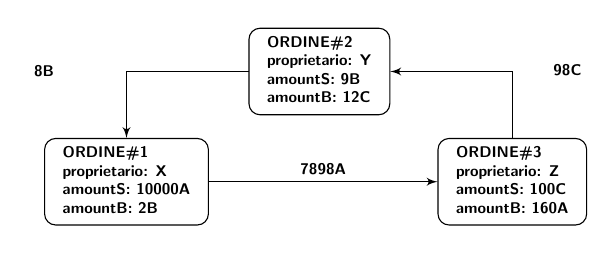
\begin{tikzpicture}[
    auto,
    node distance=2cm,
    >=latex',
    font=\bfseries\footnotesize\sffamily,
    order/.style={
		scale=0.7,
		rectangle,
		rounded corners,
		draw=black,
		text centered,
%		text width=5cm,
		minimum height=12mm,
		fill=white
	},
	label/.style={
		scale=0.7
	}
  ]
    % We start by placing the blocks

  \node [order] (order2)
 {%
 \begin{tabular}{l}
  \textbf{ORDINE\#2}\\
  \textbf{proprietario: Y}\\
  \textbf{amountS: 9B}\\
  \textbf{amountB: 12C}
 \end{tabular}
 };

  \node [order, below of=order2, xshift=-3.5cm] (order1)
 {%
 \begin{tabular}{l}
  \textbf{ORDINE\#1}\\
  \textbf{proprietario: X}\\
  \textbf{amountS: 10000A}\\
  \textbf{amountB: 2B}
 \end{tabular}
 };


  \node [order, below of=order2, xshift=3.5cm] (order3)
 {%
 \begin{tabular}{l}
  \textbf{ORDINE\#3}\\
  \textbf{proprietario: Z}\\
  \textbf{amountS: 100C}\\
  \textbf{amountB: 160A}
 \end{tabular}
 };

 \draw [draw,->] (order1) -- node [label] {\textbf{7898A}} (order3);
 \draw [draw,->] (order2) -| node [label, xshift=-1.8cm] {\textbf{8B}} (order1);
 \draw [draw,->] (order3) |- node [label, xshift=1cm, yshift=0.24cm] {\textbf{98C}} (order2);

\end{tikzpicture}

\caption{Un anello composto da 3 ordini}
\label{fig:ring}
\end{figurehere}
\end{center}


La figura 1 mostra un anello di ordini composto tra 3 ordini. Ogni token in un ordine di vendita (\verb|tokenS|) \'e anche un token in un altro ordine d'acquisto (\verb|tokenB|). Viene cos\'i creato un loop che permette ad ogni ordine di scambiare i token desiderati senza la necessit\'a di un ordine opposto per quella coppia. Gli ordini tradizionali di scambio di coppie possono, ovviamente, essere ancora essere eseguiti, in quello che \'e essenzialmente  un caso speciale di anello di ordini.


\begin{definition}[anello di ordini] Siano $C_{0}$, $C_{1}$, $\cdots$, $C_{n-1}$ $n$ differenti token, e siano $O_{0\rightarrow 1}$, $\cdots$, $O_{i\rightarrow i\oplus 1}$, $\cdots$, $O_{n-1 \rightarrow 0}$ $n$ differenti ordini. Questi ordini possono formare un anello di ordini per lo scambio:
$$O_{0\rightarrow 1} \rightarrow \cdots \rightarrow O_{i\rightarrow i\oplus 1} \rightarrow \cdots \rightarrow O_{n-1\rightarrow 0} \text{, }$$
dove $n$ \'e la lunghezza dell'anello di ordini, e $i\oplus 1 \equiv i+1 \mod n$.
\end{definition}

Un anello di ordini \'e valido quando tutte le transazioni che lo compongono possono essere eseguite ad un tasso di scambio uguale o migliore del tasso originale specificato implicitamente dall'utente. Per verificare la validit\'a dell'anello di ordini, gli smart contracts del protocollo Loopring devono ricevere gli anelli di ordini dai minatori e controllare che il prodotto dei tassi di scambio originali di tutti gli ordini \'e maggiore o uguale a 1.

Assumiamo che Alice e Bob vogliono scambiare i loro token \verb|A| e \verb|B| . Alice possiede 15 token \verb|A| vuole scambiarli con 4 token \verb|B|; Bob possiede 10 token \verb|B| vuole scambiarli con 30 token \verb|A|.

Chi sta comprando e chi sta vendendo? Ci\'o dipende esclusivamente dal bene che scegliamo di fissare per dare un prezzo alle quotazioni. Se il token \verb|A|  \'e preso come riferimento, allora Alice sta comprando un token \verb|B| al prezzo di ${15 \over 4} = 3.75$\verb|A|, mentre Bob sta vendendo 10 token \verb|B| al prezzo di ${30 \over 10} = 3.00$\verb|A|. Nel caso in cui fissassimo il token \verb|B| as reference, we say that Alice is selling 15 token \verb|A| for the price of ${4\over 15}=0.26666667$\verb|B| and Bob is buying 10 token \verb|A| for the price of ${10 \over 30}=0.33333334$\verb|B|. Hence, who's the buyer or seller is arbitrary.

Nella prima situazione Alice \'e disposta a pagare un prezzo pi\'u alto ($3.75$\verb|A|) rispetto al prezzo che Bob chiede per vendere i suoi token ($3.00$\verb|A|), mentre nella seconda situazione Bob \'e disposto a pagare un prezzo pi\'u alto ($0.33333334$\verb|B|) rispetto al prezzo a cui Alice sta vendendo i suoi token ($0.26666667$\verb|B|). \'E chiaro che uno scambio \'e possibile quando il compratore \'e disposto a pagare un prezzo uguale o maggiore di quello richiesto dal venditore.

\begin{equation}
{{15\over 4} \over {30\over 10}} = {{10\over 30} \over {4\over 15}}={15 \over 4} \cdot {10 \over 30} = 1.25 > 1
\end{equation}

Pertanto, perch\'e un insieme di $n$ ordini possano essere completati, integralmente o parzialmente, dobbiamo sapere se il prodotto tra ogni singolo tasso di scambio degli ordini d'acquisto \'e maggiore o uguale a 1. Se ci\'o avviene, tutti gli $n$ ordini possono essere completati, parzialmente o totalmente \cite{supersymmetry}.

Se aggiungiamo un terzo soggetto, Charlie, per cui Alice vuole cedere $x_1$ token \verb|A| e ricevere $y_1$ token \verb|B|, Bob vuole cedere $x_2$ token \verb|B| e ricevere $y_2$ token \verb|C|, e Charlie vuole cedere $x_3$ token \verb|C| e ricevere $y_3$ token \verb|A|.  I token necessari sono presenti, e lo scambio \'e possibile se:

\begin{equation}
{{x_1 \cdot x_2 \cdot x_3 \over y_1 \cdot y_2 \cdot y_3} \geq 1}
\end{equation}


Vedere la sezione \ref{anatomy} per maggiori dettagli sugli ordini di Loopring.



\section{Partecipanti dell'Ecosistema\label{sec:ecosystem}}
I seguenti partecipanti dell'ecosistema forniscono congiuntamente tutte le funzionalit\'a che un exchange centralizzato pu\'o offrire.

\begin{itemize}

\item \textbf{Wallets}: Un comune servizio di portafoglio o un'interfaccia che permette agli utenti di accedere ai propri token ed un modo per inviare ordini al network Loopring. I Wallets saranno incentivati a produrre ordini condividendo commissioni con i minatori di anelli  (vedere sezione \ref{sec:token}). Con la credenza che il futuro degli scambi avr\'a luogo al sicuro all'interno dei wallets degli utenti, connettere queste riserve di liquidit\'a attraverso il nostro protocollo \'e fondamentale.

\item \textbf{Blockchain del Consorzio di Condivisione di Liquidit\'a/Mesh di Rel\'e}: Un network di mesh di rel\'e per la condivisione di ordini e liquidit\'a.  I nodi che eseguono il software Loopring per rel\'e, hanno la possibilit\'a di unirsi ad un network gi\'a esistente e condividere liquidit\'a con altri rel\'e attraverso un consorzio. Il consorzio che stiamo costruendo in una prima implementazione ha un capacit\'a di condivisione ordini quasi in tempo reale (1-2 secondi per blocco), ed elimina lo storico degli ordini molto antico per permettere ai nuovi nodi di scaricare la blockchain pi\'u velocemente.
Si tenga in considerazione che i rel\'e non devono necessariamente unirsi a questo consorzio; possono agire in modo indipendente e non condividere la liquidit\'a con altri, o possono creare e gestire un loro network di condivisione di liquidit\'a.

\item \textbf{Rel\'e/Minatori di Anelli}:I Rel\'e sono nodi che ricevono ordini dai wallet o dal mesh di rel\'e, mantengono un registro di commesse ed uno storico degli scambi pubblici, ed eventualmente trasmettono ordini ad altri rel\'e (attraverso un qualunque strumento oltre alla blockchain) e/o a nodi di mesh di rel\'e. L'operazione di minare anelli \'e una caratteristica aggiuntiva - non un requisito - dei rel\'e. Questa \'e infatti computazionalmente molto intensiva ed \'e svolta completamente fuori dalla blockchain. Chiamiamo i rel\'e che minano \enquote{Ring-Miners}, in quanto producono anelli di ordini combinando insieme ordini diversi. I rel\'e sono liberi di (1) scegliere di comunicare tra di loro, (2) decidere come costruire il loro registro di commesse, e (3) scegliere quale algoritmo utilizzare per minare gli anelli di ordini.


\item \textbf{Smart Contracts del Protocollo Loopring (LPSC)}: Un insieme di smart contracts pubblici e gratuiti che controllano gli anelli di ordini ricevuti dai minatori di ordini, trasferiscono i token per conto degli utenti in modo sicuro, incentivano le operazioni dei wallets e dei minatori di anelli attraverso la creazione di commissioni, e creano eventi. I browsers di ordini/Rel\'e utilizzano questi eventi per mantenere aggiornati i propri registri ed il proprio storico di scambi. Vedere l'appendice \ref{app:protocol_ethereum} per i dettagli.

\item \textbf{Servizi di Tokenizzazione Asset (ATS)}: Un ponte tra assets che non possono essere scambiati direttamenti con Loopring. Sono servizi gestiti in modo centralizzato da imprese ed organizzazioni rispettabili. Gli utenti depositano assets (beni reali, fiat o token di altre blockchains) ed ottengono in cambio token che in futuro potranno essere nuovamente convertiti per i loro depositi. Loopring non \'e un protocollo che permette scambi tra blockchains differenti (fino a quando non verr\'a individuata una soluzione idonea), ma l'ATS permette lo scambio tra tokens ERC20 \cite{ERC20} e beni fisici, cos\'i come con beni presenti su altre blockchains.

\end{itemize}


\section{Processo di Scambio\label{sec:process}}



\begin{enumerate}


\item \textbf{Autorizzazione del Protocollo}: In figura \ref{fig:process}, l'utente \verb|Y| che vuole scambiare tokens autorizza gli LPSC a gestire \verb|amountS| del token \verb|B| the user wants to sell. che l'utente vuole vendere. Questa operazione non blocca i tokens dell'utente, che rimane libero di trasferirli mentre l'ordine viene processato.

\item \textbf{Creazione dell'Ordine}: Il tasso di cambio corrente ed il registro delle commesse per il token \verb|B| da scambiare per il token \verb|C|,  sono offerti dai rel\'e o da altri agenti connessi al network, come i browsers di ordini. L'utente \verb|Y| piazza un ordine (ordine con limite di prezzo) specificando \verb|amountS| e \verb|amountB| e altri parametri attraverso le interfacce dei wallet che integrano il protocollo. Un certo ammontare di LRx pu\'o essere aggiunto all'ordine come commissione per i minatori d'anelli; pi\'u \'e alta la commissione di LRx pi\'u \'e alta la probabilit\'a che un minatore processi rapidamente l'ordine. L'hash dell'ordine \'e firmato con la chiave privata dell'utente \verb|Y|.

\item \textbf{Trasmissione dell'Ordine}: Il wallet invia l'ordine e la sua firma digitale ad uno o pi\'u rel\'e che quindi aggiornano i propri registri pubblici delle commesse. Il protocollo non richiede che il registro sia costruito in un modo specifico, ad esempio con il metodo primo-arrivato-primo-servito. I rel\'e hanno il potere di crearlo come meglio preferiscono.

\item \textbf{Condivisione della Liquidit\'a}: I rel\'e trasmettono l'ordine agli altri rel\'e attraverso il metodo che ritengono pi\'u idoneo. Ancora una volta, c'\'e flessibilit\'a sul come/se i nodi interagiscono. Per facilitare il raggiungimento di un certo livello di connettivit\'a, \'e stato implementato un meccanismo di condivisione della liquidit\'a tra mesh di rel\'e utilizzando un consorzio. Come menzionato nella sezione precedente, questo mesh di relay \'e ottimizzato per velocit\'a ed inclusivit\'a.


\begin{center}
\begin{figurehere}
\centering
\tikzstyle{block} = [draw, fill=blue!20, rectangle,
    minimum height=3em, minimum width=6em]
\tikzstyle{sum} = [draw, fill=blue!20, circle, node distance=1cm]
\tikzstyle{input} = [coordinate]
\tikzstyle{output} = [coordinate]
\tikzstyle{pinstyle} = [pin edge={to-,thin,black}]

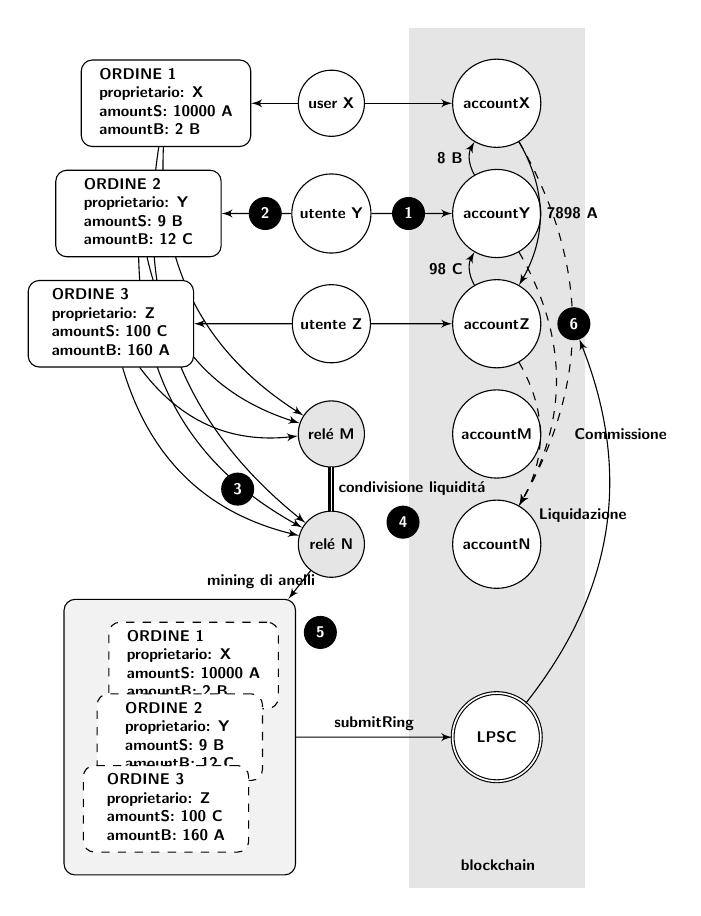
\begin{tikzpicture}[
    auto,
    scale=0.7,
    node distance=2cm,
    >=latex',
    font=\bfseries\footnotesize\sffamily,
    order/.style={
		rectangle,
		scale=0.7,
		rounded corners,
		draw=black,
		text centered,
%		text width=5cm,
		minimum height=12mm,
		minimum width=30mm,
		fill=white
	},
	role/.style={
		circle,
		scale=0.7,
		draw=black,
		text centered,
%		text width=5cm,
		minimum height=12mm,
		minimum width=12mm,
		fill=white
	},
	steps/.style={
		circle,
		scale=0.7,
		draw=black,
		text centered,
%		text width=5cm,
%		minimum height=12mm,
%		minimum width=12mm,
		fill=black,
		text=white
	},
	account/.style={
		circle,
		scale=0.7,
		draw=black,
		text centered,
%		text width=5cm,
		minimum height=16mm,
		minimum width=16mm,
		fill=white
	},
	label/.style={
	  scale=0.7
    }
  ]


 \node [role] (user1)  {user X};
 \node [role, below of=user1] (user2)  {utente Y};
 \node [role, below of=user2] (user3)  {utente Z};
 \node [role, below of=user3, fill=gray!20] (relay1)  {rel\'e M};
 \node [role, below of=relay1, fill=gray!20] (relay2)  {rel\'e N};


 \node [order, left of=user1, xshift=-1cm] (order1)
 {%
 \begin{tabular}{l}
  \textbf{ORDINE 1}\\
  \textbf{proprietario: X}\\
  \textbf{amountS: 10000 A}\\
  \textbf{amountB: 2 B}
 \end{tabular}
 };

 \draw [draw, ->]  (user1) -- (order1) [label]{};
 \draw [bend right,->] (order1) to node [auto, scale=0.7] {} (relay1);
 \draw [bend right,->] (order1) to node [auto, scale=0.7] {} (relay2);
% \draw [draw, ->]  (order1) |- (relay1) [label]{};
% \draw [draw, ->]  (order1) |- (relay2) [label]{};

 \node [order,left of=user2, xshift=-1.5cm] (order2)
 {%
 \begin{tabular}{l}
  \textbf{ORDINE 2}\\
  \textbf{proprietario: Y}\\
  \textbf{amountS: 9  B}\\
  \textbf{amountB: 12 C}
 \end{tabular}
 };
 \draw [draw, ->]  (user2) -- (order2) [label]{};
 \draw [bend right,->] (order2) to node [auto, scale=0.7] {} (relay1);
 \draw [bend right,->] (order2) to node [auto, scale=0.7] {} (relay2);
% \draw [draw, ->]  (order2) |- (relay1) [label]{};
% \draw [draw, ->]  (order2) |- (relay2) [label]{};
%
\node [order, left of=user3, xshift=-2cm] (order3)
 {%
 \begin{tabular}{l}
  \textbf{ORDINE 3}\\
  \textbf{proprietario: Z}\\
  \textbf{amountS: 100 C}\\
  \textbf{amountB: 160 A}
 \end{tabular}
 };
 \draw [draw, ->]  (user3) -- (order3) [label]{};
 \draw [bend right,->] (order3) to node [auto, scale=0.7] {} (relay1);
 \draw [bend right,->] (order3) to node [auto, scale=0.7] {} (relay2);
% \draw [draw, ->]  (order3) |- (relay1) [label]{};
% \draw [draw, ->]  (order3) |- (relay2) [label]{};

% // The Ring
\node [order,
yshift=-1.5cm,
xshift=-2.75cm,
below of=relay2,
fill=gray!10,
minimum width=4.2cm,
minimum height=5cm] (ring) {};


\node [order, dashed, below of=relay2,yshift=-0.2cm,xshift=-2.5cm] (order11)
 {%
 \begin{tabular}{l}
  \textbf{ORDINE 1}\\
  \textbf{proprietario: X}\\
  \textbf{amountS: 10000 A}\\
  \textbf{amountB: 2 B}
 \end{tabular}
 };
 \node [order, dashed,below of=order11,xshift=-0.25cm,yshift=0.7cm] (order21)
 {%
 \begin{tabular}{l}
  \textbf{ORDINE 2}\\
  \textbf{proprietario: Y}\\
  \textbf{amountS: 9  B}\\
  \textbf{amountB: 12 C}
 \end{tabular}
 };
\node [order, dashed,below of=order21,xshift=-0.25cm,yshift=0.7cm] (order31)
 {%
 \begin{tabular}{l}
  \textbf{ORDINE 3}\\
  \textbf{proprietario: Z}\\
  \textbf{amountS: 100 C}\\
  \textbf{amountB: 160 A}
 \end{tabular}
 };

 % // The blockchain
\node [
rectangle,
fill=gray!20,
right of=user1,
yshift=-4.5cm,
xshift=0.1cm,
scale=0.7,
minimum width=3.2cm,
minimum height=15.6cm] (blockchain) {\parbox[b][15cm]{1.3cm}{blockchain}};
% blockchain accounts
  \node [account, right of=user1, xshift=1cm] (account1)  {accountX};
  \node [account, right of=user2, xshift=1cm] (account2)  {accountY};
  \node [account, right of=user3, xshift=1cm] (account3)  {accountZ};
  \node [account, right of=relay1, xshift=1cm] (account4)  {accountM};
  \node [account, right of=relay2, xshift=1cm] (account5)  {accountN};
  \node [account, double, below of=account5, yshift=-1.5cm] (psc)  {LPSC};

 \draw [draw, ->]  (user1) -- (account1) [label]{};
 \draw [draw, ->]  (user2) -- (account2) [label]{};
 \draw [draw, ->]  (user3) -- (account3) [label]{};
% \draw [draw, ->]  (relay1) -- (account4) [label]{};
% \draw [draw, ->]  (relay2) -- (account5) [label]{};
 \draw [draw, double, thick]  (relay1) to node [auto, scale=0.7] {condivisione liquidit\'a}  (relay2) [label]{};
% \draw [draw, ->]  (relay1) -- (ring) [label]{};
 \draw [draw, ->]  (relay2) to node [auto, scale=0.7, xshift=-1.8cm, yshift=0.3cm] {mining di anelli}  (ring) [label]{};
 \draw [draw, ->]  (ring) to node [auto, scale=0.7] {submitRing} (psc) [label]{};

 \draw [bend left,->] (account1) to node [auto, scale=0.7] {\textbf{7898 A}} (account3);
 \draw [bend left,->] (account2) to node [auto, scale=0.7] {\textbf{8 B}} (account1);
 \draw [bend left,->] (account3) to node [auto, scale=0.7] {\textbf{98 C}} (account2);

 \draw [bend left,->, dashed] (account1) to node [auto, scale=0.7] {} (account5);
 \draw [bend left,->, dashed] (account2) to node [auto, scale=0.7] {} (account5);
 \draw [bend left,->, dashed] (account3) to node [auto, scale=0.7, xshift=.5cm] {\textbf{Commissione}} (account5);


% \draw [draw,->] (order1) -- node [label] {\textbf{7898 A}} (order3);
% \draw [draw,->] (order2) -| node [label, xshift=-1.8cm] {\textbf{8 B}} (order1);
% \draw [draw,->] (order3) |- node [label, xshift=1cm, yshift=0.24cm] {\textbf{98 C}} (order2);

\node [steps, right of=user2, xshift=-0.6cm] () {1};
\node [steps, left of=user2, xshift=0.8cm] () {2};
\node [steps, left of=relay2, xshift=0.3cm, yshift=1cm] () {3};
\node [steps, left of=relay1, xshift=3.3cm, yshift=-1.6cm] () {4};
\node [steps, below of=relay2, xshift=-0.2cm, yshift=0.4cm] () {5};
\node [steps, right of=account3, xshift=-0.6cm] (step5) {6};

 \draw [bend right, ->]  (psc) to node [auto, scale=0.7, xshift=0.5cm] {Liquidazione} (step5) [label]{};

\end{tikzpicture}

\caption{Processo di Scambio Loopring}
\label{fig:process}
\end{figurehere}
\end{center}



\item \textbf{Mining di Anelli (Abbinamento di Ordini)}: I minatori di anelli provano ad eseguire l'ordine interamente o parzialmente ad un dato tasso di scambio o ad un tasso migliore, abbinandolo a diversi altri ordini. Il mining di Anelli \'e il motivo principale per cui il protocollo \'e in grado di offrire un'alta liquidit\'a per qualunque coppia di ordini. Se il tasso a cui l'ordine \'e eseguito \'e migliore di quello specificato dall'utente \verb|Y|, il margine \'e condiviso tra tutti gli ordini che compongono l'anello. Come premio, il minatore pu\'o scegliere tra la riscossione di una parte del margine (Divisione del Margine, e ritornare agli utenti gli LRx), o semplicemente trattenere la commissione in LRx.


\item \textbf{Verifica \& Transazione}: L'anello di ordini \'e ricevuto dagli LPSC. Sono necessari diversi controlli per verificare i dati forniti dal minatore e determinare se l'anello di ordini pu\'o essere completato integralmente o parzialmente (ci\'o dipende dal tasso di completamento degli ordini nell'anello e dai token presenti nei wallet degli utenti). Se tutti i controlli hanno esito positivo, il contratto trasferisce i token agli utenti e paga i minatori e le commissioni ai wallet contemporaneamente. Se gli LPSC rilevano una mancanza di fondi necessari allo scambio nel wallet dell'utente \verb|Y|, l'ordine verr\'a ridimensionato: un ordine ridimensionato torna automaticamente alla sua dimensione originaria se un quantitativo sufficiente di fondi viene depositato all'indirizzo dell'utente, diversamente da una cancellazione, che \'e una operazione manuale a senso unico che non pu\'o essere annullata.


\end{enumerate}





%
%\end{multicols}
%
%\begin{center}
%\begin{figurehere}
%\includegraphics[height=8cm]{images/en_protocol.png}
%\caption{Loopring Trading Process}
%\label{fig: Loopringrotocol}
%\end{figurehere}
%\end{center}
%
%\begin{multicols}{2}

\section{Flessibilit\'a Operativa\label{sec:business_model}}
\'E importante notare che gli open standard di Loopring permettono ai partecipanti di operare con una significativa flessibilit\'a. Gli attori sono liberi di implementare nuovi modelli di business e generare valore per gli utenti, guadagnando commissioni in LRx  sui volumi di scambio o su altre metriche definite nel processo (se lo decidono). L'ecosistema \'e modulare e pensato per incoraggiare la partecipazione di una moltitudine di applicazioni.

\subsection{ Il Registro delle Commesse\label{sec:order_book}}
I rel\'e possono progettare i loro registri in svariati modi per combinare ed abbinare e gli ordini degli utenti. Una prima implementazione del nostro registro delle commesse segue un modello OTC, dove gli ordini a prezzo limitato sono posizionati basandosi soltanto sul prezzo. Il momento in cui sono stati generati gli ordini, in altri termini, non ha un impatto sulla formazione del registro.Tuttavia, un rel\'e \'e libero di progettare il proprio registro in modo da emulare il funzionamento tipico di exchange centralizzati, dove gli ordini sono classificati per prezzo ma rispettando anche il momento temporale di creazione dell'ordine. Se un rel\'e \'e pi\'u incline ad offrire questo tipo di meccanismo, pu\'o creare/integrarsi con un wallet, e avere che gli ordini che partono da quel wallet vengano inviati a questo singolo rel\'e, che sar\'a poi in grado di smistarli basandosi sul tempo. Ogni tipo di  configurazione \'e possibile.

Mentre altri protocolli DEX richiedono a volte che i rel\'e possiedano delle risorse - una riserva di token iniziali per piazzare gli ordini dell'acquirente - i rel\'e Loopring devono soltanto trovare ordini abbinabili per far eseguire lo scambio, e possono farlo senza risorse iniziali.

\subsection{Condivisione della Liquidit\'a\label{sec:liquidity_sharing}}
I rel\'e sono liberi di progettare come condividere la liquidit\'a (ordini) tra di loro. Il nostro consorzio \'e solo una delle soluzioni per raggiungere questo scopo, e l'ecosistema \'e libero di interagire e comunicare come desidera. Oltre ad unirsi al consorzio blockchain, \'e possibile creare e gestire nuovi consorzi, creando le regole/incentivi che si ritengono pi\'u opportuni. I rel\'e possono anche lavorare in autonomia, come visto nel caso dell'implementazione che tiene conto del tempo. Sicuramente ci sono chiari vantaggi nel comunicare con gli altri come ad esempio la ricerca dell'effetto rete, tuttavia, differenti modelli di business possono avere necessit\'a di tipologie particolari di condivisioni e di divisioni delle commissioni.


\section{Specifiche del Protocollo\label{sec:protocol}}

\subsection{Anatomia di un Ordine\label{anatomy}}
Un ordine \'e un pacchetto di dati che descrive l'intento dell'utente allo scambio. Un ordine Loopring  \'e definito utilizzando il Modello di Ordine Unidirezionale, o UDOM, come segue:

\begin{verbatim}
  message Order {
    address protocol;
    address owner;
    address tokenS;
    address tokenB;
    uint256 amountS;
    uint256 amountB;
    unit256 lrcFee
    unit256 validSince; // Seconds since epoch
    unit256 validUntil; // Seconds since epoch
    uint8   marginSplitPercentage;  // [1-100]
    bool    buyNoMoreThanAmountB;
    uint256 walletId;
    // Dual-Authoring address
    address authAddr;
   	// v, r, s are parts of the signature
    uint8   v;
    bytes32 r;
    bytes32 s;
    // Dual-Authoring private-key,
    // not used for calculating order's hash,
    // thus it is NOT signed.
    string  authKey;
  }
\end{verbatim}


Per assicurare l'origine dell'ordine, questo viene firmato contro l'hash dei suoi parametri con la chiave privata dell'utente, escludendo \verb|authAddr|. Il parametro \verb|authAddr| viene usato per firmare gli anelli d'ordine di cui lo stesso ordine \'e parte, in modo da prevenire il front-running. Si veda la sezione \ref{sec:dual_authoring} per ulteriori dettagli. La firma \'e rappresentata dai campi \verb|v|, \verb|r|, ed \verb|s| , e viene trasmessa sulla rete insieme ai parametri d'ordine. Ci\'o assicura che l'ordine rimanga invariato durante la sua intera esistenza. Nonostante l'ordine rimanga invariato, il protocollo \'e comunque in grado di calcolarne lo stato attuale sulla base dell'ammontare del suo indirizzo e di altre variabili.


UDOM non include alcun prezzo (che per natura deve essere un numero a virgola mobile), ma utilizza piuttosto il termine \verb|rate| o $r$, che viene espresso come \verb|amountS|/\verb|amountB|. Il rate non \'e un numero a virgola mobile, ma un'espressione che verr\'a solamente valutata a richiesta con altri interi non oggetto di firma, cos\'i da mantenere tutti i risultati intermedi come interi non firmati ed aumentarne l'accuratezza di calcolo.

\subsubsection{Importi d'acquisto}

Quando un minatore d'anelli crea  un anello abbinando degli ordini, \'e possibile che risulti perseguibile un rate migliore, che permetter\'a agli utenti di ottenere pi\'u \verb|tokenB| del numero \verb|amountB| che hanno specificato.  Ad ogni modo se il parametro \verb|buyNoMoreThanAmountB| \'e impostata a \verb|True|, il protocollo assicura che gli utenti ricevano un numero di \verb|amountB| non maggiore di \verb|tokenB|. Il parametro di UDOM \verb|buyNoMoreThantokenB| determina quindi quando un ordine sia da considerarsi completamente evaso. \verb|buyNoMoreThantokenB| applica un valore massimo ad \verb|amountS| o \verb|amountB|, e permette agli utenti di esprimere le proprie intenzioni di scambio in modo pi\'u granulare rispetto ai tradizionali ordini.

Per esempio: con  \verb|amountS| = 10 w \verb|amountB| = 2, il  rate $r$ = 10/2 = 5. L'utente \'e quindi intenzionato a vendere 5 \verb|tokenS| per ciascun \verb|tokenB|. Il minatore trova e fa ottenere all'utente un rate di 4, permettendogli di ricevere 2.5 \verb|tokenB| al posto di 2. Ad ogni modo, se l'utente vuole soltanto 2 \verb|tokenB| ed imposta il parametro \verb|buyNoMoreThanAmountB| a \verb|True|, gli LPSC effettuano la transazione ad un rate di 4, e l'utente vende 4 \verb|tokenS| per ogni \verb|tokenB|, con un risparmio effettivo di 2 \verb|tokenS|. Da considerare che non sono qui prese in esame le commissioni. (cf. sezione \ref{sec:fee_model}).

Quindi utilizzando


\begin{verbatim}
	      Order(amountS,tokenS,
	            amountB,tokenB,
	            buyNoMoreThantokenB)
\end{verbatim}

per rappresentare un ordine in modo semplificato, per i mercati ETH/USD di un exchange tradizionale, una normale modellazione di compravendita pu\'o gestire il 1° ed il 3° ordine riportato sotto, ma non i due rimanenti:

\begin{enumerate}
	\item Vendi 10 ETH ad un prezzo di 300 USD/ETH. Questo può esprimersi come: \verb|Order(10, ETH, 3000, USD, False)|.
	\item Vendi  ETH  ad un prezzo di 300  USD/ETH  per ottenere  3000  USD.  Questo pu\'o esprimersi come: \verb|Order(10, ETH, 3000, USD, True)|.
	\item Compra 10 ETH ad un prezzo di 300 USD/ETH, Questo pu\'o esprimersi come: \verb|Order(3000, USD, 10, ETH, True)|.
	\item Spendi 3000  USD  per comprare quanti pi\'u  ETH possibile ad un prezzo di 300  USD/ETH,  Questo pu\'o esprimersi come: \verb|Order(3000, USD, 10, ETH, False)|.
\end{enumerate}



\subsection{Verifica dell'anello\label{sec:ring_verification}}

Gli Smart  Contracts  del protocollo Loopring non calcolano il rate di scambio o gli  importi, ma devono ricevere e verificare cosa i minatori forniscono come tali valori. Queste computazioni vengo effettuate dai minatori essenzialmente per due motivazioni principali: (1) il linguaggio di programmazione degli smart contracts, come solidity\cite{dannen2017introducing} nel caso di Ethereum, non supporta il calcolo a virgola mobile, specialmente  pow(x, 1/n)  (calcolare la radice n-esima di un numero a  virgola mobile), (2)  \'e auspicabile che tale calcolo avvenga off-chain cos\'i da ridurre le operazioni ed il costo di utilizzo della blockchain.


\subsubsection{Verifica del Sub-Ring\label{sec:sub_ring_check}}
Questo passaggio inibisce agli arbitraggisti la possibilit\'a di ottenere in modo scorretto l'intero margine di un anello d'ordine, mediante la creazione di nuovi ordini al suo interno. Sostanzialmente, una volta che un minatore identifica un anello d'ordine valido, potrebbe cadere nella tentazione di aggiungere ulteriori ordini allo stesso anello, cos\'i da assorbire il margine dell'utente (tasso di sconto). Come illustrato nella sottostante figura \ref{fig:subring}, calcolando opportunamente x1, y1, x2 e y2 sar\'a possibile rendere il prodotto di tutti i rate d'ordine pari ad 1, cos\'i da annullare qualsiasi tasso di scambio.

\begin{center}
\begin{figurehere}
\centering
\tikzstyle{block} = [draw, fill=blue!20, rectangle,
    minimum height=3em, minimum width=6em]
\tikzstyle{sum} = [draw, fill=blue!20, circle, node distance=1cm]
\tikzstyle{input} = [coordinate]
\tikzstyle{output} = [coordinate]
\tikzstyle{pinstyle} = [pin edge={to-,thin,black}]

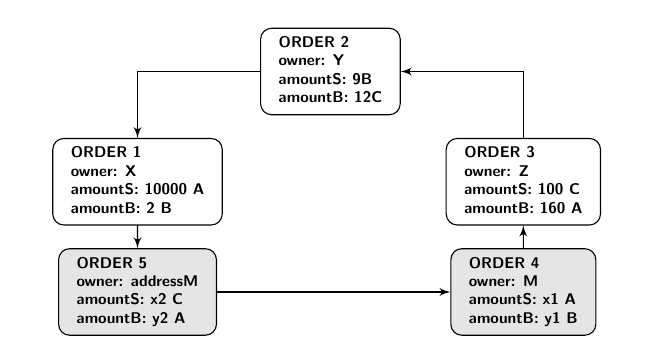
\begin{tikzpicture}[
    auto,
    node distance=2cm,
    >=latex',
    font=\bfseries\footnotesize\sffamily,
    order/.style={
		scale=0.7,
		rectangle,
		rounded corners,
		draw=black,
		text centered,
%		text width=5cm,
		minimum height=12mm,
		fill=white
	},
	label/.style={
		scale=0.7
	}
  ]
    % We start by placing the blocks

  \node [order] (order2)
 {%
 \begin{tabular}{l}
  \textbf{ORDER 2}\\
  \textbf{owner: Y}\\
  \textbf{amountS: 9B}\\
  \textbf{amountB: 12C}
 \end{tabular}
 };

  \node [order, below of=order2, xshift=-3.5cm] (order1)
 {%
 \begin{tabular}{l}
  \textbf{ORDER 1}\\
  \textbf{owner: X}\\
  \textbf{amountS: 10000 A}\\
  \textbf{amountB: 2 B}
 \end{tabular}
 };


  \node [order, below of=order2, xshift=3.5cm] (order3)
 {%
 \begin{tabular}{l}
  \textbf{ORDER 3}\\
  \textbf{owner: Z}\\
  \textbf{amountS: 100 C}\\
  \textbf{amountB: 160 A}
 \end{tabular}
 };

   \node [order, below of=order3, fill=gray!20] (order4)
 {%
 \begin{tabular}{l}
  \textbf{ORDER 4}\\
  \textbf{owner: M}\\
  \textbf{amountS: x1 A}\\
  \textbf{amountB: y1 B}
 \end{tabular}
 };


  \node [order, below of=order1, fill=gray!20] (order5)
 {%
 \begin{tabular}{l}
  \textbf{ORDER 5}\\
  \textbf{owner: addressM}\\
  \textbf{amountS: x2 C}\\
  \textbf{amountB: y2 A}
 \end{tabular}
 };

 \draw [draw,->] (order1) -- node [label, xshift=-2cm] {} (order5);
 \draw [draw,->] (order2) -| node [label, xshift=-1.6cm] {} (order1);
 \draw [draw,->] (order3) |- node [label, xshift=1cm] {} (order2);
 \draw [draw,->] (order4) -- node [label, xshift=1.8cm] {} (order3);
 \draw [draw,->] (order5) -- node [label, yshift=0.2cm] {} (order4);

\end{tikzpicture}

\caption{Un anello d'ordine con un sotto-anello}
\label{fig:subring}
\end{figurehere}
\end{center}

Ci\'o comporta zero rischi, non apporta alcun valore aggiunto al network, ed \'e da considerarsi pertanto un comportamento scorretto da parte del minatore.  Per prevenire questa possibilit\'a, Loopring impone che un loop valido non possa contenere alcun sotto-anello.  Per verificare questa condizione, gli LPSC fanno in modo che ogni token non possa comparire pi\'u di una volta in posizione di acquisto o vendita. Nel diagramma sopra, possiamo vedere come il token \verb|A| compaia due volte  come token d'acquisto e altrettante come token di vendita, questo non sarebbe pertanto permesso.


\subsubsection{Verifica del Tasso di Completamento\label{sec:fill_rate_check}}


Il calcolo del tasso di scambio nell'anello d'ordine \'e svolto dai minatori per le motivazioni sopra esposte. Gli LPSC devono verificarne la correttezza. Innanzitutto verificano che il tasso d'acquisto eseguibile dal minatore per ciascun ordine sia minore o uguale al tasso d'acquisto imposto dall'utente. Questo assicura che l'utente ottenga nella transazione almeno il tasso di scambio richiesto, se non migliore.
A seguito della conferma dei tassi di scambio, gli LPSC assicurano che ciascun ordine che compone l'anello benefici dello stesso sconto. Ad esempio, se il tasso di sconto \'e $\gamma$, allora il prezzo per ogni ordine sar\'a:

$r_{0\rightarrow 1} \cdot (1-\gamma)$, $r_{1\rightarrow 2} \cdot (1-\gamma)$, $r_{2 \rightarrow 0} \cdot (1-\gamma)$, e soddisfer\'a:
\begin{equation}
r_{0\rightarrow 1} \cdot (1-\gamma)\cdot r_{1\rightarrow 2} \cdot (1-\gamma) \cdot r_{2 \rightarrow 0} \cdot (1-\gamma) = 1
\end{equation}
da cui:
\begin{equation}
\gamma = 1- \frac{1}{\sqrt[3]{r_{0\rightarrow 1} \cdot r_{1\rightarrow 2} \cdot r_{2\rightarrow 0}}}\text{.}
\end{equation}
Se la transazione aggrega $n$ ordini, allora lo sconto \texttt{discount} \'e:
\begin{equation}
\gamma = 1- \frac{1}{\sqrt[n]{\prod_{i=0}^{n-1} r^i}} \text{,}
\end{equation}

dove $r^i$ rappresenta il tasso di scambio dell'ordine $i$-esimo. Ovviamente, solamente quando lo sconto \'e $\gamma \ge 0$, questi ordini possono esser soddisfatti; ed il tasso di scambio dell'ordine $i$-esimo  ($O^i$) \'e $\hat{r^i} = r^i \cdot (1-\gamma)$, $\hat{r^i}\le r^i$.

Ricordiamo il nostro esempio precedente in cui Alice ha 15 token \verb|A| e vuole scambiarli con \verb|B|, e Bob ha 10 token \verb|B| e vuole scambiarli con 20 token \verb|A|. Se il token \verb|A| \'e preso come riferimento, allora Alice sta comprando token \verb|B| per $\frac{15}{4}$ = 3.75\verb|A|, mentre Bob sta vendendo token \verb|B| per $\frac{30}{10}$ = 3.00\verb|A|. Per calcolare lo sconto: $\frac{150}{120}$ = 1.25 da cui $\frac{1}{1.25}$ = 0.8 = $(1 −- \gamma)^2$. Da qui, il tasso di scambio che rende equa la transazione per entrambe le parti \'e $\sqrt{0.8}$ $\cdot$ 3.75 $\approx$ 3.3541 token \verb|A| per ogni token \verb|B|.

Bob ha 4 token \verb|B| e riceve 13.4164 token \verb|A|,  pi\'u dei 12 che si aspettava di ottenere. Alice riceve i 4 token \verb|B| che si aspettava ma li paga solo 13.4164 token \verb|A|, meno dei 15 che era disposta a pagare. Si noti che una frazione di questo margine verr\'a utilizzata per pagare le commissioni che servono ad incentivare i minatori (e i wallet). (Vedere la sezione  \ref{sec:fee_model}).


\subsubsection{Tracciamento del completamento \& cancellazione}

Un utente pu\'o cancellare parzialmente o completamente un ordine mediante l'invio di una specifica transazione agli LPSC, contenente i dettagli dell'ordine e l'importo da cancellare. Gli LPSC ne prendono atto, registrano l'importo da cancellare ed emettono al network un evento \verb|OrderCancelled| Gli LPSC tengono e traccia di importi eseguiti e cancellati tramite un registro che utilizza l'hash dell'ordine come identificativo. Questi dati sono accessibili pubblicamente e gli eventi di \verb|OrderCancelled| ed \verb|OrderFilled| vengono emessi ad ogni variazione. Il tracciamento di questi valori rappresenta qualcosa di critico per gli LPSC nel processo di evasione dell'anello d'ordine.

Gli LPSC supportano inoltre la cancellazione di un ordine per qualsiasi coppia di scambio attraverso l'evento \verb|OrdersCancelled| e la cancellazione di tutti gli ordini relativi ad un indirizzo tramite l'evento \verb|AllOrdersCancelled|.


\subsubsection{Scaling degli ordini\label{sec:order_scaling}}
Gli ordini vengono riscalati in base all'esistenza di precedenti importi storici transati o cancellati, nonch\'e sulla base del saldo degli account emittenti. Il processo identifica sulla base di queste caratteristiche l'ordine da eseguire con l'importo minore e lo utilizza come riferimento per ordinare tutte le transazioni dell'anello d'ordine.
L'identificazione dell'ordine caratterizzato dal minor valore agevola la stima del volume d'esecuzione di ogni ordine. Ad esempio, supponendo che l'ordine $i$-esimo sia quello caratterizzato dal minor valore, il numero di token venduti per ogni ordine $\hat{s}$ ed il numero di token acquistati $\hat{b}$ per ogni ordine pu\'o essere calcolato come:

\[
\begin{split}
&\hat{s}^{i}=\overline{s}_i\text{, } \hat{b}^{i}=\hat{s}^{i}/ \hat{r}^i\text{, }\text{;}\\
&\hat{s}^{i\oplus 1}=\hat{b}^i\text{, } \hat{b}^{i\oplus 1}=\hat{s}^{i\oplus 1}/ \hat{r}^{i\oplus 1}\text{;}\\
&\hat{s}^{i\oplus 2}=\hat{b}^{i\oplus 1}\text{, } \hat{b}^{i\oplus 2}=\hat{s}^{i\oplus 2}/ \hat{r}^{i\oplus 2}\text{;}\\
& ...
%\text{.}
\end{split}
\]
dove $\overline{s}_i$ \'e il saldo rimanente dopo che gli ordini sono stati parzialmente eseguiti.

In fase d'implementazione, possiamo tranquillamente assumere che qualunque ordine dell'anello abbia il minor valore, e quindi iterare nell'anello al massimo due volte per calcolare il volume d'esecuzione di ciascun ordine.

Esempio: Se il minor importo da soddisfare rappresenta il 5\%, dell'ordine originale, tutte le transazioni dell'anello saranno ridotte del 5\%. Una volta che le transazioni sono completate, l'ordine che si considerava avesse l'importo minore ancora da soddisfare dovr\'a  risultare completamente eseguito.

\subsection{Liquidazione dell'anello\label{sec:settlement}}

Se l'anello d'ordine soddisfa tutti i punti precedenti, lo stesso pu\'o essere chiuso cos\'i da permettere l'esecuzione delle transazioni. Ci\'o significa che tutti gli $n$ ordini formeranno un anello chiuso, connesso come in figura 4:

\begin{center}
\begin{figurehere}
\centering
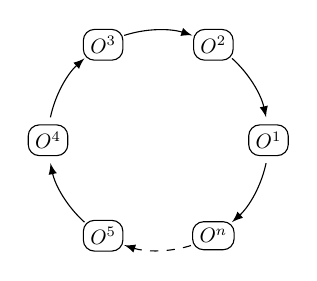
\begin{tikzpicture}[
circle/.style={
		scale=0.75,
		rounded corners,
		draw=black,
		text centered,
		}
]

\def \n {6}
\def \m {4}
\def \radius {1.4cm}
\def \margin {12} % margin in angles, depends on the radius

\foreach \s in {1,...,\m}
{
  \node[draw, circle] at ({360/\n * (\s - 1)}:\radius) {$O^\s$};
  \draw[<-, >=latex] ({360/\n * (\s - 1)+\margin}:\radius)
    arc ({360/\n * (\s - 1)+\margin}:{360/\n * (\s)-\margin}:\radius);
}

\node[draw, circle] at ({360/\n * 4}:\radius) {$O^5$};
  \draw[<-, dashed, >=latex] ({360/\n * 4+\margin}:\radius)
    arc ({360/\n * 4+\margin}:{360/\n * (5)-\margin}:\radius);

\node[draw, circle] at ({360/\n * 5}:\radius) {$O^n$};
  \draw[<-, >=latex] ({360/\n * 5+\margin}:\radius)
    arc ({360/\n * 5+\margin}:{360/\n * (6)-\margin}:\radius);


\end{tikzpicture}
\caption{Liquidazione dell'anello}
\label{fig:settlement}
\end{figurehere}
\end{center}

Per effettuare le transazioni, gli LPSC utilizzano lo smart contract \verb|TokenTransferDelegate| .L'introduzione di tale preposto rende pi\'u semplice l'upgrade di qualsiasi smart contract del protocollo, in quanto tutti gli ordini dovranno soltanto autorizzare quest'ultimo anzich\'e gestire le differenti versioni del protocollo.
Per ogni ordine dell'anello, il pagamento di \verb|tokenS| viene effettuato con il successivo od il precedente ordine, a seconda dell'implementazione. Quindi la commissione del minatore viene versata in funzione del modello di commissioni scelto dal minatore stesso. Infine, una volta che tutte le transazioni sono effettuate, viene emesso l'evento \verb|RingMined|.

\subsubsection{Eventi emessi\label{sec:events}}

Il protocollo emette eventi che permettono ai rel\'e, ai gestori d'ordine e ad altri attori coinvolti di ricevere aggiornamenti sul registro delle commesse in modo pi\'u efficiente possibile. Questi eventi sono:

\begin{itemize}
	\item \textbf{OrderCancelled}: Un ordine specifico \'e stato cancellato.
	\item \textbf{OrdersCancelled}: Tutti gli ordini provenienti da un singolo indirizzo per una specifica coppia di scambio sono stati cancellati.
	\item \textbf{AllOrdersCancelled}: Tutti gli ordini provenienti da un singolo indirizzo sono stati cancellati.
	\item \textbf{RingMined}: Un anello d'ordine \'e stato correttamente liquidato. Questo evento contiene i dati relativi ad ogni singolo trasferimento di token all'interno dell'anello.
\end{itemize}


\section{LRx Token\label{sec:token}}
LRx \'e la nostra notazione generica di token. LRC \'e il token Loopring su Ethereum, LRQ su Qtum, LRN su NEO, etc. Altre tipologie di LRx saranno introdotte in futuro, man mano che Loopring verr\'a esteso ad altre blockchain pubbliche.

\subsection{Modello di Commissioni\label{sec:fee_model}}
Quando gli utenti creano un ordine, specificano un importo di LRx da versare al minatore come commissione, oppure una percentuale del margine ottenuto tramite l'ordine (\verb|marginSplitPercentage|)  che il minatore pu\'o richiedere, definito margin split. Spetta al minatore la decisione su quale opzione applicare tra commissione o margin split.

Qui una rappresentazione del margin split:

\begin{center}
\begin{figurehere}
\centering
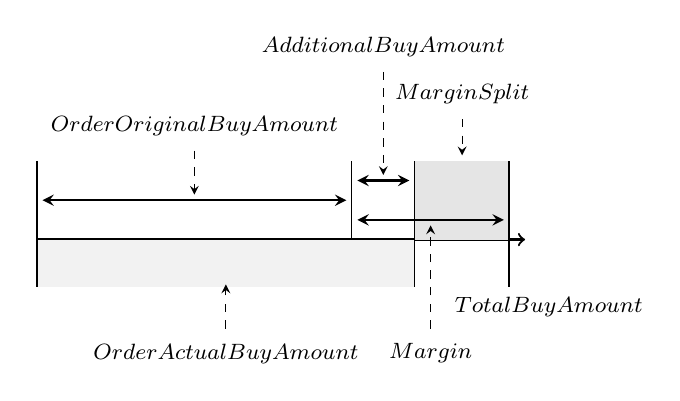
\begin{tikzpicture}[
scale=1,
font=\bfseries\footnotesize\sffamily,
classical/.style={thick,<->,shorten >=2pt,shorten <=2pt,>=stealth},
oneway/.style={->,dashed,shorten >=2pt,shorten <=2pt,>=stealth}
]
    % Draw axes
    \draw [->,thick] (0,1) node (yaxis) [above] {$$}
        |- (6.2,0) node (xaxis) [right] {$$};

    \draw
  	(4,0) coordinate (A)
  	(4,1) coordinate (A2)
  	(4.8,-0.6) coordinate (B)
  	(4.8,1) coordinate (B2)
  	(6,-0.6) coordinate (C)
  	(6,1) coordinate (C2);

  	\fill [draw=none, fill=gray!20]
    (4.8, 0) rectangle (6, 1);

  	\fill [draw=none, fill=gray!10]
    (0, -0.6) rectangle (4.8, 0);
	\draw[thick] (0, -0.6) -- (0, 0.6) node[below]{$$};
  	\draw[thick, thin] (A) -- (A2) node[below]{$$};
  	\draw[thick, thin] (B) -- (B2) node[below]{$$};
  	\draw[thick] (C) node[below, xshift=0.5cm]{$Total Buy Amount$} -- (C2) ;

  	\draw[classical] (0, 0.5) -> (4, 0.5) node[below]{$$};
  	\draw[classical] (4, 0.75) -> (4.8, 0.75) node[below]{$$};
%  	\draw[classical] (4.8, 0.5) -> (6, 0.5) node[below]{$$};
  	\draw[classical] (4, 0.25) -> (6, 0.25) node[below]{$$};

  	\draw[oneway] (2, 1.2) node[above]{$Order Original Buy Amount$} -- (2, 0.5);
  	\draw[oneway] (4.4, 2.2) node[above]{$Additional Buy Amount$} -- (4.4, 0.75);
  	\draw[oneway] (5.4, 1.6) node[above]{$Margin Split$} -- (5.4, 1);
  	\draw[oneway] (5, -1.2) node[below]{$Margin$} -- (5, 0.25);
  	\draw[oneway] (2.4, -1.2) node[below]{$Order Actual Buy Amount$} -- (2.4, -0.5);
\end{tikzpicture}
\caption{A 60\% Margin Split}
\label{fig:marginsplit}
\end{figurehere}
\end{center}
Se il margine sull'anello di ordini \'e troppo contenuto, il minatore propender\'a per la commissione in LRx. Se, al contrario, il margine \'e tale da rendere conveniente il margin-split rispetto alla commissione in LRx, il minatore propender\'a per il margin split. Si applica però un'ulteriore condizione: quando il minatore propende per il margin split, questo dovr\'a versare all'utente che ha creato l'ordine una commissione almeno pari al numero di LRx che l'utente avrebbe dovuto versare come commissione al minatore. Ci\'o eleva di fatto la soglia a partire da cui il minatore potr\'a considerare l'adozione del margin split a due volte la commissione in LRx, aumentando di fatto la propensione verso l'adozione della commissione in LRx. Questo permette ai minatore di ottenere un compenso fisso su anelli di ordini a margine ridotto, ottenendo allo stesso tempo un compenso inferiore su anelli di ordini con margine pi\'u alto.
Il nostro modello di commissione si basa sull'aspettativa che, con la crescita e maturazione del mercato, ci sar\'a un numero sempre inferiore di anelli di ordini con alto margine, da cui la necessit\'a di incentivare una commissione fissa in LRx. Otteniamo pertanto il seguente grafico:

\begin{center}
\begin{figurehere}
\centering
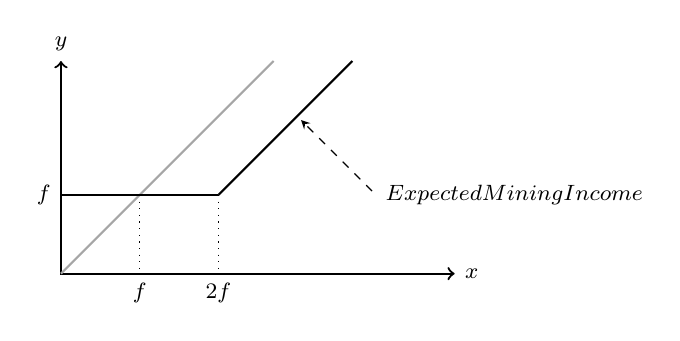
\begin{tikzpicture}[
font=\bfseries\footnotesize\sffamily,
oneway/.style={->,dashed,shorten >=2pt,shorten <=2pt,>=stealth},
scale=1]
    % Draw axes
    \draw [<->,thick] (0,2.7) node (yaxis) [above] {$y$}
        |- (5,0) node (xaxis) [right] {$x$};

    \draw
  	(1,1) coordinate (A)
  	(2,1) coordinate (B);


  	\draw[thick] (B) -- (3.7,2.7);
  	\draw[dotted] (B) -- (2,0) node[below] {$2f$};
  	\draw[dotted] (A) -- (1,0) node[below] {$f$};
  	\draw[thick,color=gray!70] (0,0) -- (2.7,2.7);
  	\draw[thick] (0,1) node[left] {$f$}--(B) node[     ]{$$};
 	\draw[oneway] (4,1) node[right]{$Expected Mining Income$} -- (3, 2);
\end{tikzpicture}
\caption{Modello di commissioni di Loopring}
\label{fig:feemodel}
\end{figurehere}
\end{center}
dove $f$ \'e la commissione in LRx, $x$ \'e il margin split, $y$  \'e il compenso del minatore. $y=max(f, x-f)$ come indicato dalla linea continua; se la commissione in LRx per l'ordine \'e $0$, l'equazione diviene $y=max(0, x - 0)$ che si semplifica in $y=x$ come indicato dalla linea in grigio.
Queste le conseguenze:
\begin{enumerate}
	\item Se il margin split \'e 0, i minatori propenderanno per la commissione fissa in LRx, traendone comunque incentivo.
	\item Se la commissione in LRx \'e 0,  il risultato \'e un modello generico lineare come rappresentato dalla linea in grigio.
	\item Quando il guadagno da il margin  split  \'e maggiore di 2x(LRx  fee), i minatori  sceglieranno il margin split, versando la commissione in LRx all'utente.
\end{enumerate}
Da notare che se la commissione in LRx \'e diversa da zero, a prescindere dall'opzione adottata dal minatore, vi sar\'a comunque un trasferimento di LRx tra il minatore ed il creatore dell'ordine. In un caso il minatore guadagna la commissione in LRx, nell'altro versa la stessa commissione in LRx al creatore d'ordine, propendendo per il margin split.
I minatori condivideranno una certa percentuale del compenso con i gestori di wallet. Quando un utente piazza un ordine attraverso un wallet e questo viene eseguito, il gestore di wallet viene compensato con una porzione della commissione o del margin split.

Nonostante questo approccio sia modulare, e sia possibile implementare il proprio modello a riguardo, consideriamo che la percentuale di commissioni da condividere con i wallet sia approssimativamente del 20\%-25\%. I wallet rappresentano infatti un target chiave per l'implementazione del protocollo Loopring, avendo una propria base utenti, e potendo al momento contare su limitate fonti di guadagno.

\subsection{Governance decentralizzata}
Il protocollo Loopring \'e nel suo fondamento un protocollo social, nel senso che si affida sulla coordinazione di diversi attori per permettere loro di collaborare in modo efficiente verso un goal comune. Ci\'o non \'e dissimile da altri protocolli che caratterizzano la Cryptoeconomia in senso lato, la cui utilit\'a \'e ampiamente regolata dagli stessi meccanismi dei problemi di coordinamento \cite{vitalikgovernance}, equilibrio d'attivazione e razionalit\'a limitata. A questo fine, i token LRx non sono solamente intesi per il pagamento di commissioni, ma bens\'i per allineare gli incentivi finanziari dei diversi partecipanti del network. Questo allineamento \'e una condizione fondamentale per l'adozione di qualsiasi protocollo, ma ancor di pi\'u per i protocolli di scambio, considerando che il successo di quest'ultimi \'e determinato dalla capacit\'a di migliorare la liquidit\'a di un ecosistema decentralizzato.

I token LRx saranno utilizzati per permettere di gestire i futuri aggiornamenti del protocollo tramite governance decentralizzata. Gli aggiornamenti degli smart contracts saranno governati dai possessori di token cos\'i da assicurarne continuit\'a e sicurezza, mitigando i rischi di eccessiva liquidit\'a, non compatibile. L'immutabilit\'a degli smart contracts una volta rilasciati, costituisce un rischio che le dApps o gli utenti finali continuino ad interagire con version deprecate, e ne precludano l'aggiornamento.
La possibilit\'a di aggiornamento \'e chiave per il successo di un protocollo, che deve potersi adattare dinamicamente alla richiesta del mercato e sottostanti blockchain. Una governance decentralizzata da parte dei possessori di LRx permetter\'a l'aggiornamento degli smart contracts del protocollo senza compromettere dApps o utenti finali, o senza affidarsi eccessivamente all'astrazione degli smart contracts. I token LRx esistono in quantit\'a limitate, e nel caso degli LRC, una percentuale di questi sono tenuti bloccati dalla Fondazione Loopring ed allocati in fondi speciali diretti alla comunit\'a \cite{LRCtokendoc}.

Tuttavia, i possessori dei token LRx non sono i soli portatori di interessi da considerare nell'evoluzione da imprimere al protocollo: rel\'e/minatori, wallet, sviluppatori ed altri sono parte integrante dell'ecosistema e la loro voce deve essere ascoltata. Infatti, dato che questi agenti non hanno la necessit\'a di possedere alcun LRx per svolgere il loro rispettivo lavoro (dato che i market makers e i makers/takers tradizioni non esistono, le riserve iniziali non sono obbligatorie) dobbiamo mettere in atto metodi alternativi per rispettare i loro interessi.  Inoltre, il “semplice” voto basato sui token, sia on-chain che off-chain, \'e una soluzione imperfetta, perch\'e la concentrazione della propriet\'a ed un basso turnout di voto pongono dei rischi. Da ci\'o, l'obiettivo \'e quello di implementare un modello di governance che \'e costruito su diversi livelli, e che poggia sulla consapevolezza che un certo insieme di processi decisionali sono la normalit\'a. Questo pu\'o essere facilitato da istituti di coordinamento che offrono segnali da diversi insiemi di partecipanti, e forse, da punti focali stabiliti a priori. Man mano che il sistema diventer\'a operativo, la Fondazione Loopring evolver\'a inevitabilmente da un insieme di sviluppatori di protocollo ad assistenti di protocollo.

\section{Protezione dagli Attacchi e dalle Frodi}
\subsection{Prevenzione del Front-running\label{sec:dual_authoring}}
Negli exchange decentralizzati, il front-running avviene quando qualcuno prova a copiare l'ordine di scambio di un altro nodo, e a farlo minare prima della transazione originale, che si trova in attesa nell'insieme delle transazioni (mempool). Questa azione pu\'o essere attuata specificando una commissione di transazione pi\'u alta (prezzo di gas). Il principale schema di front-running in Loopring (e in qualunque protocollo di abbinamento ordini) \'e il furto di ordini (order-flitch): quando un front-runner ruba uno o pi\'u ordini di un anello da una transazione pendente; e specificatamente riguardo Loopring: quando un front-runner ruba un intero anello d'ordini da una transazione pendente.
Quando una transazione submittRing non \'e stata confermata ed \'e ancora nell'insieme delle transazioni pendenti, chiunque pu\'o facilmente individuare queste transazioni e sostituire \verb|minerAddress| con il loro  indirizzo (il \verb|filcherAddress|), cos\'i facendo, possono firmare nuovamente il pacchetto dati con \verb|filcherAddress| tper sostituire la firma dell'anello d'ordini. Il ladro pu\'o fissare un prezzo di gas pi\'u alto e inviare una nuova transazione sperando che i minatori prenderanno la sua nuova transazione all'interno del prossimo blocco invece della transazione submitRing originale.
Le soluzioni precedentemente trovate a questo problema presentavano considerevoli aspetti negativi: richiedendo pi\'u transazioni e quindi aumentando i costi di gas per i minatori;  e prendendo almeno il doppio dei blocchi per fissare un anello. La nostra nuova soluzione, il Dual Authoring \cite{dualauthor}, implica l'adozione di un meccanismo che mette a punto due livelli di autorizzazione per gli ordini – uno per il regolamento, ed uno per il mining dell'anello.

Il processo di Dual Authoring:
\begin{enumerate}
	\item Per ogni ordine, il wallet generer\'a una coppia di chiave pubblica/chiave privata casuale, la coppia di chiavi verr\'a inserita nel JSON snippet dell'ordine. (Un'alternativa \'e quella di usare l'indirizzo derivato dalla chiave pubblica invece che la chiave pubblica di per s\'e per ridurre la dimensione in termini di byte. Utilizziamo \verb|authAddr| per rappresentare questo indirizzo, e \verb|authKey|  per raffigurare la combaciante chiave privata \verb|authAddr|).
	\item Viene calcolato l'hash dell'ordine con tutti i campi all'interno dell'ordine (ad eccezione di \verb|r|, \verb|v|, \verb|s|, e \verb|authKey|),e viene firmato l'hash utilizzando la chiave privata del proprietario \verb|owner| (non \verb|authKey|).
	\item Il wallet mander\'a l'ordine insieme a \verb|authKey|  ai rel\'e per essere minato. I minatori verificheranno che \verb|authKey| e \verb|authAddr| sono abbinate correttamente e che la firma dell'ordine \'e valida rispetto all'indirizzo del proprietario.
	\item Quando un anello \'e stato identificato, i minatori useranno \verb|authKey| dell'ordine per firmare l'hash dell'anello,  il  \verb|minerAddress|, e tutti i parametri del mining. Se un order-ring contiene $n$ ordini, ci saranno conseguentemente, $n$ firme da $n$ \verb|authKey|s. Abbiamo nominato queste firme come \verb|authSignature|s. Il minatore potrebbe anche aver bisogno di firmare l'hash dell'anello insieme a tutti i parametri del mining utilizzando la chiave privata del \verb|minerAddress|.
	\item  Il minatore richiama la funzione submitRing con tutti i parametri, e allo stesso tempo tutte le extra \verb|authSignature|s. È importante notare che \verb|authKey|s  NON \'e parte delle transazioni on-chain e quindi rimangono sconosciute ad altre parti ad eccezione del minatore.
	\item Il protocollo di Loopring verificher\'a ognuna delle \verb|authSignature| rispetto al corrispondente \verb|authAddr| di ogni ordine, e rifiuter\'a l'order-ring se qualcuna delle \verb|authSignature|  \'e mancante o invalida.

\end{enumerate}
Il risultato \'e che adesso:
\begin{itemize}
	\item  La firma dell'ordine (grazie alla chiave privata dell'indirizzo dell' \verb|owner|) garantisce che l'ordine non possa essere modificato, incluso il \verb|authAddr|.
	\item  La firma del minatore (grazie alla  chiave privata del \verb|minerAddress|), se fornita garantisce che nessuno possa utilizzare la sua identit\'a per minare un anello d'ordini.
	\item  La \verb|authSignature|s garantisce che l'intero anello non possa essere modificato, incluso i \verb|minerAddress|, e quindi nessun ordine pu\'o essere rubato.
\end{itemize}
Il Dual Authoring previene il furto d'ordini ed il furto di anello e nel frattempo assicura che il regolamento dell'anello possa essere eseguito in un'unica transazione. Ulteriormente, la Dual Authoring apre le porte per la trasmissione di ordini condivisi in due modi: condivisioni che non combaciano e condivisioni che combaciano.  Da condizione predefinita Loopring utilizza un modello OTC e supporta solamente ordini a prezzo limitato, ci\'o vuol dire che le marche temporali (timestamps) degli ordini vengono ignorate. Questo implica che il front-running non ha nessun impatto sul prezzo reale di quello scambio, ma ha un impatto solo se viene eseguito o no.
\section{Altri Attacchi}
\subsection{Attacchi Sybil o DOS}
Utenti malintenzionati -- operando in chiaro o sotto falsa identit\'a -- potrebbero mandare un grande numero di piccoli ordini per attaccare i nodi di Loopring. Tuttavia, visto che i nodi hanno il potere di creare da s\'e le regole sulla base delle quali accettare o rifiutare gli ordini -- informazioni che possono rendere pubbliche o mantenere private -- la maggior parte di questi ordini sarebbe rigettata per via dell'incapacit\'a di produrre profitti soddisfacenti quando abbinati. Dando il potere ai rel\'e di decidere le proprie modalit\'a di gestione degli ordini non riteniamo che un attacco con molti piccoli ordini possa essere una reale minaccia.
\subsection{Saldo Insufficiente}
Utenti in malafede potrebbero firmare e diffondere ordini il cui valore dell'ordine non \'e zero ma il cui indirizzo ha effettivamente un saldo pari a zero. I nodi potrebbero monitorare e notare che alcuni ordini hanno un saldo attuale di zero, aggiornare lo stato di questi ordini di conseguenza e quindi scartarli.
I nodi spendono tempo per aggiornare lo stato di un ordine, ma possono anche scegliere di minimizzare lo sforzo attraverso, per esempio, una lista nera di indirizzi e interrompendo i relativi ordini.
\section{Riepilogo}
Il protocollo di Loopring vuole essere una base fondamentale per gli exchange decentralizzati. Cos\'i facendo, il protocollo ha delle profonde ripercussioni in come le persone scambiano valori e beni. Il denaro, come bene intermediario, facilita o sostituisce il baratto risolvendo la problematica comunione di necessit\'a \cite{unenumerated2006}, per cui due controparti devono desiderare i rispettivi  beni o servizi. Similmente, il protocollo Loopring si pone l'obiettivo di liberarci da questa dinamica di necessit\'a di corrispondenza tra beni che si vogliono scambiare, utilizzando gli anelli come modo per facilitare gli scambi. Ci\'o \'e significativo per il modo in cui la societ\'a e i mercati scambiano tokens, beni tradizionali, e altro. Infatti, cos\'i come le criptovalute decentralizzate pongono una minaccia al controllo delle nazioni sulla moneta, un protocollo combinatorio che pu\'o mettere insieme traders (consumatori/produttori) su ampia scala, \'e una minaccia teorica al concetto stesso di moneta.
Tra i benefici del protocollo vi sono:
\begin{itemize}
	\item La gestione degli ordini off-chain e regolamento degli scambi on-chain, questo significa nessun sacrificio in termini di prestazione per la sicurezza.
	\item Grande liquidit\'a dovuta al mining di anelli e alla condivisione degli ordini.
	\item La Dual Authoring risolve il dannoso problema del front running subito oggi da tutti i DEXs e dai loro utenti.
	\item Smart contracts aperti e pubblici consentono a qualunque dApp di costruire o interagire con il protocollo.
	\item La standardizzazione tra operatori consente effetti di rete e migliora l'esperienza dell'utente.
	\item Il network mantiene flessibilit\'a nella gestione del registro delle commesse e nella comunicazione.
	\item La riduzione delle barriere di entrata, ci\'o si traduce in dire costi minori per i nodi che partecipano al network e per gli utilizzatori finali.
	\item Scambi anonimi effettuati direttamente dai portafogli degli utenti.
\end{itemize}
\section{ Ringraziamenti}
Vorremmo esprimere la nostra gratitudine ai nostri mentori, consulenti e a tutte le persone nella community che sono state cos\'i disponibili e generosi a condividere la loro conoscenza. In particolare vorremmo ringraziare Shuo Bai (di ChinaLedger); il Professore Haibin Kan; Alex Cheng, Hongfei Da; Yin Cao; Xiaochuan Wu; Zhen Wang, Wei Yu, Nian Duan, Jun Xiao, Jiang Qian, Jiangxu Xiang, Yipeng Guo, Dahai Li, Kelvin Long, Huaxia Xia, Jun Ma, and Encephalo Path per aver corretto e averci consigliato in merito a questo progetto.
\bibliography{whitepaper}
\bibliographystyle{unsrt}
\end{multicols}
\begin{appendices}
\section{Implementazione di Loopring su EVM\label{app:protocol_ethereum}}
\begin{center}
\begin{figurehere}
\centering
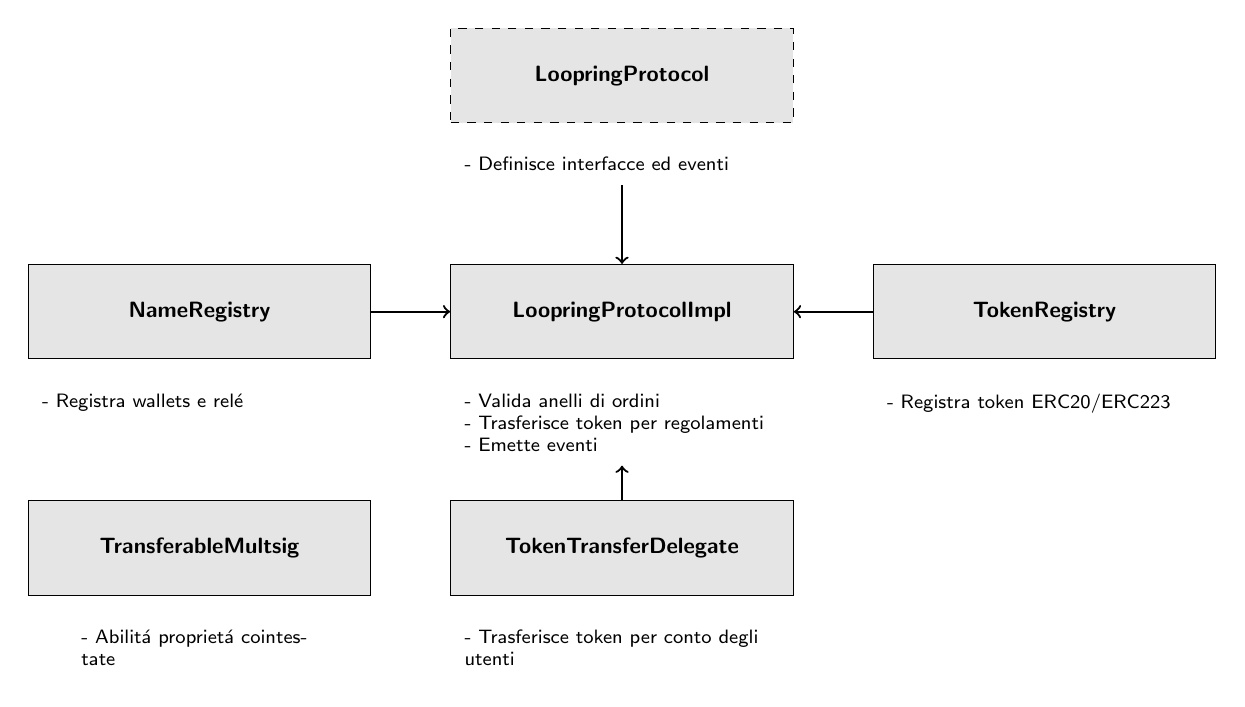
\begin{tikzpicture}
[node distance = 1cm, auto,font=\footnotesize,
% STYLES
every node/.style={node distance=3cm},
% The comment style is used to describe the characteristics of each force
comment/.style={rectangle, inner sep= 5pt, text width=4cm, node distance=0.25cm, font=\scriptsize\sffamily},
% The force style is used to draw the forces' name
force/.style={rectangle, draw, fill=black!10, inner sep=5pt, text width=4cm, text badly centered, minimum height=1.2cm, font=\bfseries\footnotesize\sffamily}]
% Draw forces
\node [force] (impl) {LoopringProtocolImpl};
\node [force, dashed, above of=impl] (protocol_interface) {LoopringProtocol};
\node [force, left=1cm of impl] (nameregistry) {NameRegistry};
\node [force, right=1cm of impl] (tokenregistry) {TokenRegistry};
\node [force, below of=impl] (delegate) {TokenTransferDelegate};
\node [force, left=1cm of delegate] (multisig) {TransferableMultsig};
%%%%%%%%%%%%%%%
% Change data from here
% impl
\node [comment, below=0.25 of impl] (comment-impl) {- Valida anelli di ordini\\
- Trasferisce token per regolamenti\\
- Emette eventi};
% nameregistry
\node [comment, below=0.25cm of nameregistry]{- Registra wallets e rel\'e};
% protocol_interface
\node [comment, below=0.25 of protocol_interface](comment-interface) {- Definisce interfacce ed eventi};
% tokenregistry
\node [comment, below=0.25 of tokenregistry] {- Registra token ERC20/ERC223};
% delegate
\node [comment, below=0.25 of delegate] {- Trasferisce token per conto degli utenti};
% PUBLIC POLICIES
\node [comment, text width=3cm, below=0.25 of multisig] {- Abilit\'a propriet\'a cointestate};
%%%%%%%%%%%%%%%%
% Draw the links between forces
\path[->,thick]
(comment-interface) edge (impl)
(nameregistry) edge (impl)
(tokenregistry) edge (impl)
(delegate) edge (comment-impl);
\end{tikzpicture}
\caption{Smart Contracts}
\label{fig:smartcontracts}
\end{figurehere}
\end{center}
\section{Distribuzione}
\subsection{Ethereum}
I seguenti smart contract sono operativi sul network Ethereum:
\begin{itemize}
\item LRC: \verb|0xEF68e7C694F40c8202821eDF525dE3782458639f|
\item TokenRegistry: \verb|0xa21c1f2AE7f721aE77b1204A4f0811c642638da9|
\item TokenTransferDelegate: \verb|0x7b126ab811f278f288bf1d62d47334351dA20d1d|
\item NameRegistry: \verb|0xd181c1808e3f010F0F0aABc6Fe1bcE2025DB7Bb7|
\item LoopringProtocolImpl: \verb|0x0B48b747436f10c846696e889e66425e05CD740f|
\end{itemize}
\subsection{Qtum}
I seguenti smart contract sono operativi sul network Qtum:
\begin{itemize}
\item LRQ: \verb| 2eb2a66afd4e465fb06d8b71f30fb1b93e18788d |
\item TokenRegistry: \verb| c89ea34360258917daf3655f8bec5550923509b3 |
\item TokenTransferDelegate: \verb| 60b3fa7f461664e4dafb621a36ac2722cc680f10 |
\item NameRegistry: \verb| e26a27d92181069b25bc7283e03722f6ce7678bb |
\item LoopringProtocolImpl: \verb| 5180bb56b696d16635abd8dc235e0ee432abf25d |
\end{itemize}
\end{appendices}
\end{document}
